\documentclass[twoside]{article}
\setlength{\oddsidemargin}{0.25 in}
\setlength{\evensidemargin}{-0.25 in}
\setlength{\topmargin}{-0.6 in}
\setlength{\textwidth}{6.5 in}
\setlength{\textheight}{8.5 in}
\setlength{\headsep}{0.75 in}
\setlength{\parindent}{0 in}
\setlength{\parskip}{0.1 in}
\newcommand{\eqdef}{:\mathrel{\mathop=}}
\newcommand{\norm}[1]{\left\lVert #1 \right\rVert}
\def\Inf{\operatornamewithlimits{inf\vphantom{p}}}

%
% ADD PACKAGES here:
%

\usepackage{amsmath,amsfonts,graphicx}

%
% The following commands set up the lecnum (lecture number)
% counter and make various numbering schemes work relative
% to the lecture number.
%
\newcounter{lecnum}
\renewcommand{\thepage}{\thelecnum-\arabic{page}}
\renewcommand{\thesection}{\thelecnum.\arabic{section}}
\renewcommand{\theequation}{\thelecnum.\arabic{equation}}
\renewcommand{\thefigure}{\thelecnum.\arabic{figure}}
\renewcommand{\thetable}{\thelecnum.\arabic{table}}
\newcommand{\indep}{\raisebox{0.05em}{\rotatebox[origin=c]{90}{$\models$}}}

%
% The following macro is used to generate the header.
%
\newcommand{\lecture}[4]{
   \pagestyle{myheadings}
   \thispagestyle{plain}
   \newpage
   \setcounter{lecnum}{#1}
   \setcounter{page}{1}
   \noindent
   \begin{center}
   \framebox{
      \vbox{\vspace{2mm}
    \hbox to 6.28in { {\bf Advanced Machine Learning
	\hfill Fall 2020} }
       \vspace{4mm}
       \hbox to 6.28in { {\Large \hfill Lecture #1: #2  \hfill} }
       \vspace{2mm}
       \hbox to 6.28in { {\it  #3 \hfill  #4} }
      \vspace{2mm}}
   }
   \end{center}
   \markboth{Lecture #1: #2}{Lecture #1: #2}

   {\bf Note}: {\it LaTeX template courtesy of UC Berkeley EECS dept.}

   {\bf Disclaimer}: {\it These notes are adapted from ETH's Advanced Machine Learning Course, ETH's Statistical Learning Theory Script and "An Introduction to Computational Learning Theory" book.}
   \vspace*{4mm}
}
%
% Convention for citations is authors' initials followed by the year.
% For example, to cite a paper by Leighton and Maggs you would type
% \cite{LM89}, and to cite a paper by Strassen you would type \cite{S69}.
% (To avoid bibliography problems, for now we redefine the \cite command.)
% Also commands that create a suitable format for the reference list.
\renewcommand{\cite}[1]{[#1]}
\def\beginrefs{\begin{list}%
        {[\arabic{equation}]}{\usecounter{equation}
         \setlength{\leftmargin}{2.0truecm}\setlength{\labelsep}{0.4truecm}%
         \setlength{\labelwidth}{1.6truecm}}}
\def\endrefs{\end{list}}
\def\bibentry#1{\item[\hbox{[#1]}]}

%Use this command for a figure; it puts a figure in wherever you want it.
%usage: \fig{NUMBER}{SPACE-IN-INCHES}{CAPTION}
\newcommand{\fig}[3]{
			\vspace{#2}
			\begin{center}
			Figure \thelecnum.#1:~#3
			\end{center}
	}
% Use these for theorems, lemmas, proofs, etc.
\newtheorem{theorem}{Theorem}[lecnum]
\newtheorem{lemma}[theorem]{Lemma}
\newtheorem{proposition}[theorem]{Proposition}
\newtheorem{claim}[theorem]{Claim}
\newtheorem{corollary}[theorem]{Corollary}
\newtheorem{definition}[theorem]{Definition}
\newenvironment{proof}{{\bf Proof:}}{\hfill\rule{2mm}{2mm}}

% **** IF YOU WANT TO DEFINE ADDITIONAL MACROS FOR YOURSELF, PUT THEM HERE:

\newcommand\E{\mathbb{E}}

\begin{document}
%FILL IN THE RIGHT INFO.
%\lecture{**LECTURE-NUMBER**}{**DATE**}{**LECTURER**}{**SCRIBE**}
\lecture{12}{PAC Learning}{}{}
%\footnotetext{These notes are partially based on those of Nigel Mansell.}

% **** YOUR NOTES GO HERE:

% Some general latex examples and examples making use of the
% macros follow.  
%**** IN GENERAL, BE BRIEF. LONG SCRIBE NOTES, NO MATTER HOW WELL WRITTEN,
%**** ARE NEVER READ BY ANYBODY.


\section{Introduction} % Don't be this informal in your notes!
The aim of the probably approximately correct (PAC) learning
model is to provide a framework for the classification problem that is distribution
independent, thus avoiding the density estimation task, in the spirit of V.N.Vapnik: “Don’t solve a harder problem than necessary”. In this section the PAC model is
presented. \\ \\
The classification problem can be formalized using the following ideas: Let $\mathbf{\mathcal{X}}$ denote the \textbf{instance} space, that is the space that encodes the objects in the learners
(algorithm) world, a \textbf{concept} over $\mathbf{\mathcal{X}}$ is defined as a subset $\mathbf{c} \subset \mathbf{\mathcal{X}}$ of the instance
space or equivalently as a function $c : \mathbf{\mathcal{X}} \to \{0, 1\}$.\\ A \textbf{concept class} is a collection of concepts. For instance $\mathbf{\mathcal{X}}$
can be the set of all possible configurations of a pixel array and the concept class of
“$A$” can be the subset of configurations that represent the letter A.\\ \\
The \textbf{set of samples} or data is defined as a subset $\mathbf{\mathcal{Z}} = \{(x_{i}
, y_{i}) : 1 \leq i \leq n \} \subset \mathbf{\mathcal{X}} \times \{0, 1\}$ where $n$ is
the number of samples and $\{0, 1\}$ is the set of labels that denotes negative or positive
examples.\\
A \textbf{classifier} is a function $c : \mathbf{\mathcal{X}}  \to \{0, 1\}$ from the instance space
to the label space. When the classifier has been trained under a specific set of samples it will be denoted by $\hat{c}_{n}$, where the $n$ specifies the number of sample points used. Finally, an \textbf{hypothesis class} is another set of concepts that we use to learn a target concept from the concept class.

\begin{definition}
Let $\mathbf{\mathcal{H}}$ and $c$ be an hypothesis class and a concept. A \textbf{learning algorithm} is an algorithm that receives as input a labeled sample $\mathbf{\mathcal{Z}} = \{(x_{i}
, y_{i}) : 1 \leq i \leq n, \;  \forall i \; y_{i} = c(x_{i}) \} $ and outputs an hypothesis $\hat{c} \in \mathbf{\mathcal{H}}$
\end{definition}

\begin{definition}
A learning algorithm $\mathbf{\mathcal{A}}$ can learn a concept $c \in \mathbf{\mathcal{C}}$ if there is a polynomial function $poly(\ldots)$ such that for any distribution $\mathbf{\mathcal{D}}$ on $\mathbf{\mathcal{X}}$ and for any $0 < \epsilon <\dfrac{1}{2}$ and $0 < \delta <\dfrac{1}{2}$: \\
if $\mathbf{\mathcal{A}}$ receives as input a sample $\mathbf{\mathcal{Z}}$ of size $n \geq poly\Big(\dfrac{1}{\epsilon},\dfrac{1}{\delta},size(\mathcal{X})\Big)$, then $\mathbf{\mathcal{A}}$ outputs $\hat{c}$ such that:
$$\mathbf{\mathbb{P}}_{\mathcal{Z} \sim \mathcal{D}^n}\Big(\mathcal{R}(\hat{c}) \leq \epsilon \Big) \geq 1- \delta$$
\end{definition}

First notice that the distribution of the data is arbitrary but fixed, therefore if a concept class is
known to be PAC learnable, no matter how pathological the distribution $\mathbf{\mathcal{D}}$ might
be in applications, the $\epsilon$,$ \delta$ guarantees will hold. \\
Second the concept class $\mathbf{\mathcal{C}}$ is fixed
and known to the algorithm designer in advance, but the target concept $c \in $ $\mathbf{\mathcal{C}}$ that
needs to be learned is not and the algorithm must be designed such that it works for
any concept in the class.\\
Third, if an algorithm requires resources (samples, time)
that scale polynomial in $\dfrac{1}{\epsilon}$ 
and $\dfrac{1}{\delta}$ where $\epsilon$ and $\delta$ are known respectively as the \textbf{error}
and \textbf{confidence} parameters, then it is said that the concept class of the problem is
\textbf{PAC efficient}.

\begin{definition}
A concept class $\mathbf{\mathcal{C}}$ is PAC learnable from a hypothesis class $\mathbf{\mathcal{H}}$ if there is an algorithm that can learn every concept $ c \in \mathbf{\mathcal{C}}$.
\end{definition}

 \section{Rectangle Learning}

The idea of the game is to learn, or find, an
unknown rectangle that is aligned with the Cartesian axes in the $\mathbb{R}^2$
space. For this
task the player can request an oracle to provide points $(x_{i}
, y_{i})$, that are distributed
according to a fixed but unknown distribution $\mathbf{\mathcal{D}}$ , and are labeled as positive if they are inside the unknown rectangle and negative in the opposite case. In the language
of the PAC definition, the instance space is the euclidean plane $\mathbf{\mathcal{X}}= \mathbb{R}^2$, the concept
class is the set of all possible axis-aligned rectangles and a concept is just one specific
rectangle from the concept class (see Fig. 12.1). The classification rule or hypothesis
$h$ formulated by the player is tested by comparing its predictions against those of
the oracle.\\ \\ 
\begin{figure}[h]
\centering

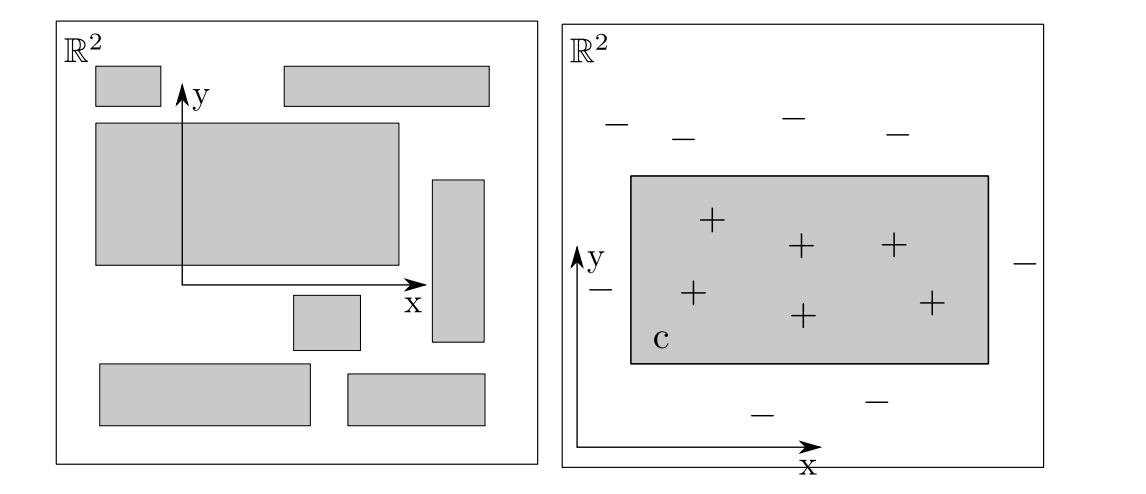
\includegraphics[width=0.4\textwidth]{img/pac1.png}
\caption{(Left) A depiction of the concept class of axis aligned rectangles in the instance
space $\mathcal{X} = \mathbb{R}^2$. (Right) Illustration of a particular concept $c$ from the concept class and
the associated training data, observe that every data point inside the rectangle (concept) is
labeled as positive and that the player must find the closest approximation to c.}
\end{figure}

A simple strategy to approach this task is known as the “tightest fitting rectangle”. The idea is to request $n$ data points from the oracle and from those that are labeled as positive built the largest possible rectangle that encloses them, without enclosing any negative point (see Fig. 12.2 Left).
\begin{figure}[h]
\centering
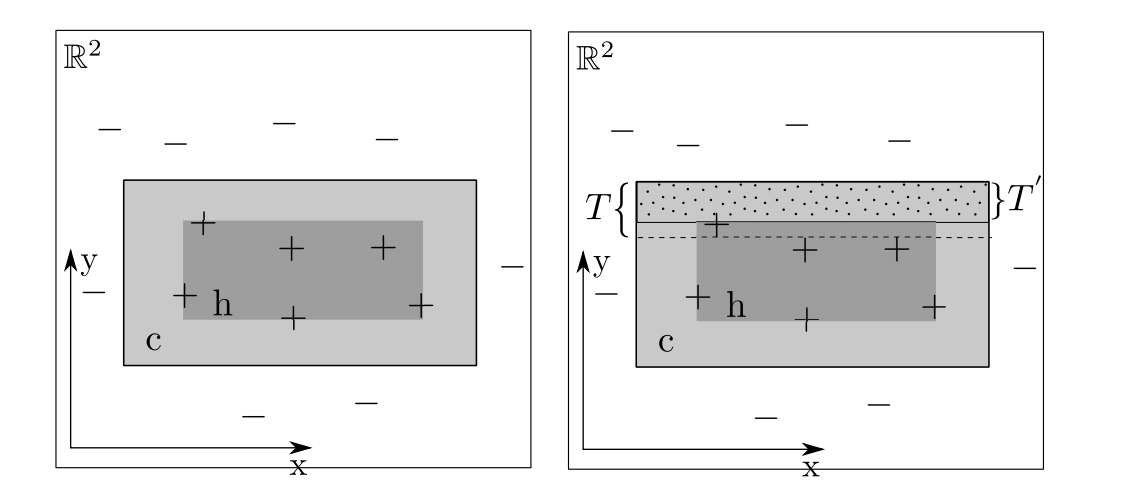
\includegraphics[width=0.4\textwidth]{img/pac2.png}
\caption{(Left) Tightest fitting rectangle hypothesis h (dark shaded rectangle) (Right)
Construction for the error analysis of the tightest fitting rectangle strategy.}
\end{figure}

Formally, we measure the error of $\hat{R}$ as the probability that a randomly chosen point from $\mathcal{D}$ falls in the region $R \Delta \hat{R}$. In our learning game, we allow the distribution $\mathcal{D}$ to be arbitrary, but we assume that is fixed, and that each example is drawn \textbf{independently} from this distribution. We will now show that the tightest-fit rectangle algorithm $\mathcal{A}$ can learn any concept $ R \in \mathcal{C}$.\\\\

First, observe that the tightest-fit rectangle $\hat{R}$ is always contained in the target rectangle $R$ and so $R \Delta \hat{R} = R - \hat{R}$. We can express the difference $R-\hat{R}$ as the union of four rectangular strips. For instance, the topmost of these strips, which is shaded and denoted $T'$ in Figure 12.2, is the region above  the upper boundary of $R$. Note that there is some overlap between these four rectangular strips at the corner.\\ Now if we can guarantee that the weight under $\mathcal{D}$ of each strip (that is the probability with respect to $\mathcal{D}$ of falling in the strip) is at most $\epsilon/4$, then we can conclude that the error of $\hat{R}$ is at most $\epsilon$. (Here we have erred on the side of pessimism by counting each overlap region twice).\\\\
Let us analyze the weight of the top strip $T'$. Define T to be the rectangular strip along the inside top of $R$ which encloses exactly weight $\epsilon/4$ under $\mathcal{D}$ (thus we sweep the top edge of $R$ downward until we have swept out weight $\epsilon/4$, see Figure 12.2). Clearly, $T'$
has weight exceeding $\epsilon/4$ under $\mathcal{D}$ if and only if $T'$ includes $T$. Furthermore, $T'$ includes $T$ if and only if no point in $T$ appears in the sample $\mathcal{Z}$ - since if $\mathcal{Z}$ does contain a point $p \in T$, this point has a positive label since it is contained in $R$, and then by construction  $\hat{R}$ must extend upwards into $T$ to cover $p$.\\\\
By definition, the probability that a single draw from the distribution $\mathcal{D}$ misses the region $T$ is exactly $1- \epsilon / 4$. Therefore, the probability that $n$ independent draws from $\mathcal{D}$ all miss the region $T$ is exactly $(1-\epsilon/4)^n$. The same analysis holds for the other three rectangular regions, so by the union bound, the probability that any of the four strips of $R \Delta \hat{R}$ has weight greater than $\epsilon/4$ is at most $4(1-\epsilon/4)^n$.\\\\
Provided that we choose $n$ to satisfy $4(1-\epsilon/4)^n \leq \delta$, then with probability $1-\delta$ over the $n$ random examples, the weight of the error region $R \Delta \hat{R}$ will be bounded by $\epsilon$, as claimed.\\ Using the inequality $(1-x) \leq e^{-x}$:
$$4 \; (1-\epsilon/4)^n \leq 4 \; e^{-n\epsilon/4} \leq \delta$$
Finally solving for $n$:

$$n \geq \dfrac{4}{\epsilon} \; \dfrac{4}{\delta} \geq \dfrac{4}{\epsilon} \log{\dfrac{4}{\delta}}$$

In summary, provided our tightest-fit algorithm takes a sample of at least $n \geq 4/\epsilon \; 4/\delta$ examples to form its hypothesis rectangle $\hat{R}$, we can assert that with probability at least $1-\delta$, $\hat{R}$ will misclassify a new point with probability at most $\epsilon$.\\\\
A few briefs comment are appropriate. First, note that the analysis does hold for any fixed probability distribution. We only needed the independence of successive point to obtain the bound. Second, the sample size bound behaves as we might expect, in that as we increase our demands - that is, as we ask for greater \textbf{accuracy} by decreasing $\epsilon$ or greater \textbf{confidence} by decreasing $\delta$ - our algorithm requires more examples to meet those demands. Finally, the algorithm we analyzed is PAC efficient: the required sample size is a slowly growing function of $1/\epsilon$ and $1/\delta$.
\newpage
\section{Error probability for realizable finite hypothesis classes}

\begin{theorem}
Let $\mathcal{C}$ be a finite concept class and assume that $\mathcal{H}$ = $\mathcal{C}$. Let $\mathcal{A}$ be an algorithm that returns a consistent hypothesis $\hat{c}$ (i.e. , $\forall n < \infty : \hat{\mathcal{R}_{n}}(\hat{c})=0)$ for any target concept $c \in \mathcal{C}$ and any i.i.d. sample $\mathcal{Z}$. For any $\epsilon, \delta >0$ if :
$$ n \geq \dfrac{1}{\epsilon}\Big(log{|\mathcal{H}|} + log{\dfrac{1}{\delta}}\Big)$$
Then the error probability is bounded by:

$$\mathbb{P}(\mathcal{R}(\hat{c})> \epsilon) \leq \delta $$
\end{theorem}

\begin{proof}\\ \\
$$\mathbb{P}\Big(\mathcal{R}(\hat{c})> \epsilon\Big) \leq \mathbb{P}\Big( \exists \hat{c}: \; \mathcal{R}(\hat{c}) > \epsilon,\; \hat{\mathcal{R}}_{n}(\hat{c}) = 0\Big) \leq \sum_{\hat{c}:\mathcal{R}(\hat{c}) > \epsilon}\mathbb{P}\Big(\mathcal{R}_{n}(\hat{c}) =0 \Big)$$

$$\leq |\mathcal{C}| \; \Big  (1-\mathcal{R}(\hat{c})\Big)^n \leq |\mathcal{C}| \; (1-\epsilon)^n \leq |\mathcal{C}| \; e^{-n \epsilon} \leq \delta$$

In particular, if we want
this probability to be smaller than some $\delta > 0$, it would suffice to let\\ $n > \dfrac{1}{\epsilon} \big(\log{|\mathcal{C}|}+  log(1/\delta) \big)$.
\end{proof}

\section{The General PAC-learning model}
In general, an instance label is not determined by the underlying concept. This is modeled with a distribution $\mathcal{D}$ on $\mathcal{X} \times \{0,1\}$ and reflects the fact that two instances with identical features might have different labels. The training set $\mathcal{Z}$ is therefore a sample from $\mathcal{D}$. Our goal is to find a hypothesis $\hat{c} \in \mathcal{H}$ with small generalization error $\mathcal{R}(\hat{c})$. \\ \\
However, if the optimal classifier is not an element of the hypothesis class, then it is impossible to attain $ \forall  \; 0  < \epsilon < 1/2: \mathcal{R}(\hat{c}) \leq \epsilon$. Instead, we aim to obtain the best possible solution i.e.,
$$\mathcal{R}(\hat{c}) - \inf_{c \in \mathcal{C}}{\mathcal{R}(c) \leq \epsilon}$$

\begin{definition}
A learning algorithm $\mathbf{\mathcal{A}}$ can learn a concept $c \in \mathbf{\mathcal{C}}$ if there is a polynomial function $poly(\ldots)$ such that for any distribution $\mathbf{\mathcal{D}}$ on $\mathbf{\mathcal{X}}$ and for any $0 < \epsilon <\dfrac{1}{2}$ and $0 < \delta <\dfrac{1}{2}$: \\
if $\mathbf{\mathcal{A}}$ receives as input a sample $\mathbf{\mathcal{Z}}$ of size $n \geq poly\Big(\dfrac{1}{\epsilon},\dfrac{1}{\delta},size(\mathcal{X})\Big)$, then $\mathbf{\mathcal{A}}$ outputs $\hat{c}$ such that:
$$\mathbf{\mathbb{P}}_{\mathcal{Z} \sim \mathcal{D}^n}\Big(\mathcal{R}(\hat{c}) - \inf_{c \in \mathcal{C}}{\mathcal{R}(c)} \leq \epsilon \Big) \geq 1- \delta$$
\end{definition}
\newpage

\section{Vapnik-Chervonenkis Inequality}

Theorem 12.4 made two restrictive assumptions:
\begin{itemize}
    \item First, there exists a perfect hypothesis (realizability). What happens when the
problem is not realizable (all hypotheses make some error)? 
\item Second, the hypothesis class is finite. What happens when the number of hypotheses is infinite? We can’t just apply a union bound any more. To answer
this, we need to have more suitable ways of measuring the “size” of a set other
than cardinality. 
\end{itemize}

Breaking free of these restrictive assumptions, we will show how bounding expected
risk can be reduced to one of uniform convergence. Recall that our goal is to bound
the excess risk, the amount by which ERM’s (empirical-risk-minimizer) expected risk exceeds the lowest possible
expected risk:
$$\mathbb{P}[\mathcal{R}(\hat{c})- \mathcal{R}(c^*)] \leq \delta$$

\begin{theorem} The following bound holds:\\ \\
$\mathbb{P}\Big[\mathcal{R}(\hat{c}) - \inf_{c \in \mathcal{C}}{\mathcal{R}(c)} > \epsilon \Big] \leq \mathbb{P}\Big[ \sup_{c \in  \mathcal{C}}{|\mathcal{R}(c)- \mathcal{\hat{R}}_{n}(c) | > \epsilon/2} \Big]$
\end{theorem}

\begin{proof}
$$\mathcal{R}(\hat{c})- \inf_{c \in \mathcal{C}}{\mathcal{R}(c)} \leq \mathcal{R}(\hat{c})- \mathcal{\hat{R}}_{n}(\hat{c})+
\mathcal{\hat{R}}_{n}(\hat{c}) - \mathcal{R}(c^*)$$
$$\leq \sup_{c \in  \mathcal{C}}{|\mathcal{R}(c)- \mathcal{\hat{R}}_{n}(c)|} + \sup_{c \in  \mathcal{C}}{|\mathcal{R}(c)- \mathcal{\hat{R}}_{n}(c) |}$$
$$\leq 2\sup_{c \in  \mathcal{C}}{|\mathcal{R}(c)- \mathcal{\hat{R}}_{n}(c)|}$$
\end{proof}

On the LHS is a statement about excess risk, and on the RHS is a statement about
uniform convergence. The RHS is the probability of the event that the largest difference
between the empirical and expected risk is at least $\epsilon/2$.
\begin{figure}[h]
\centering
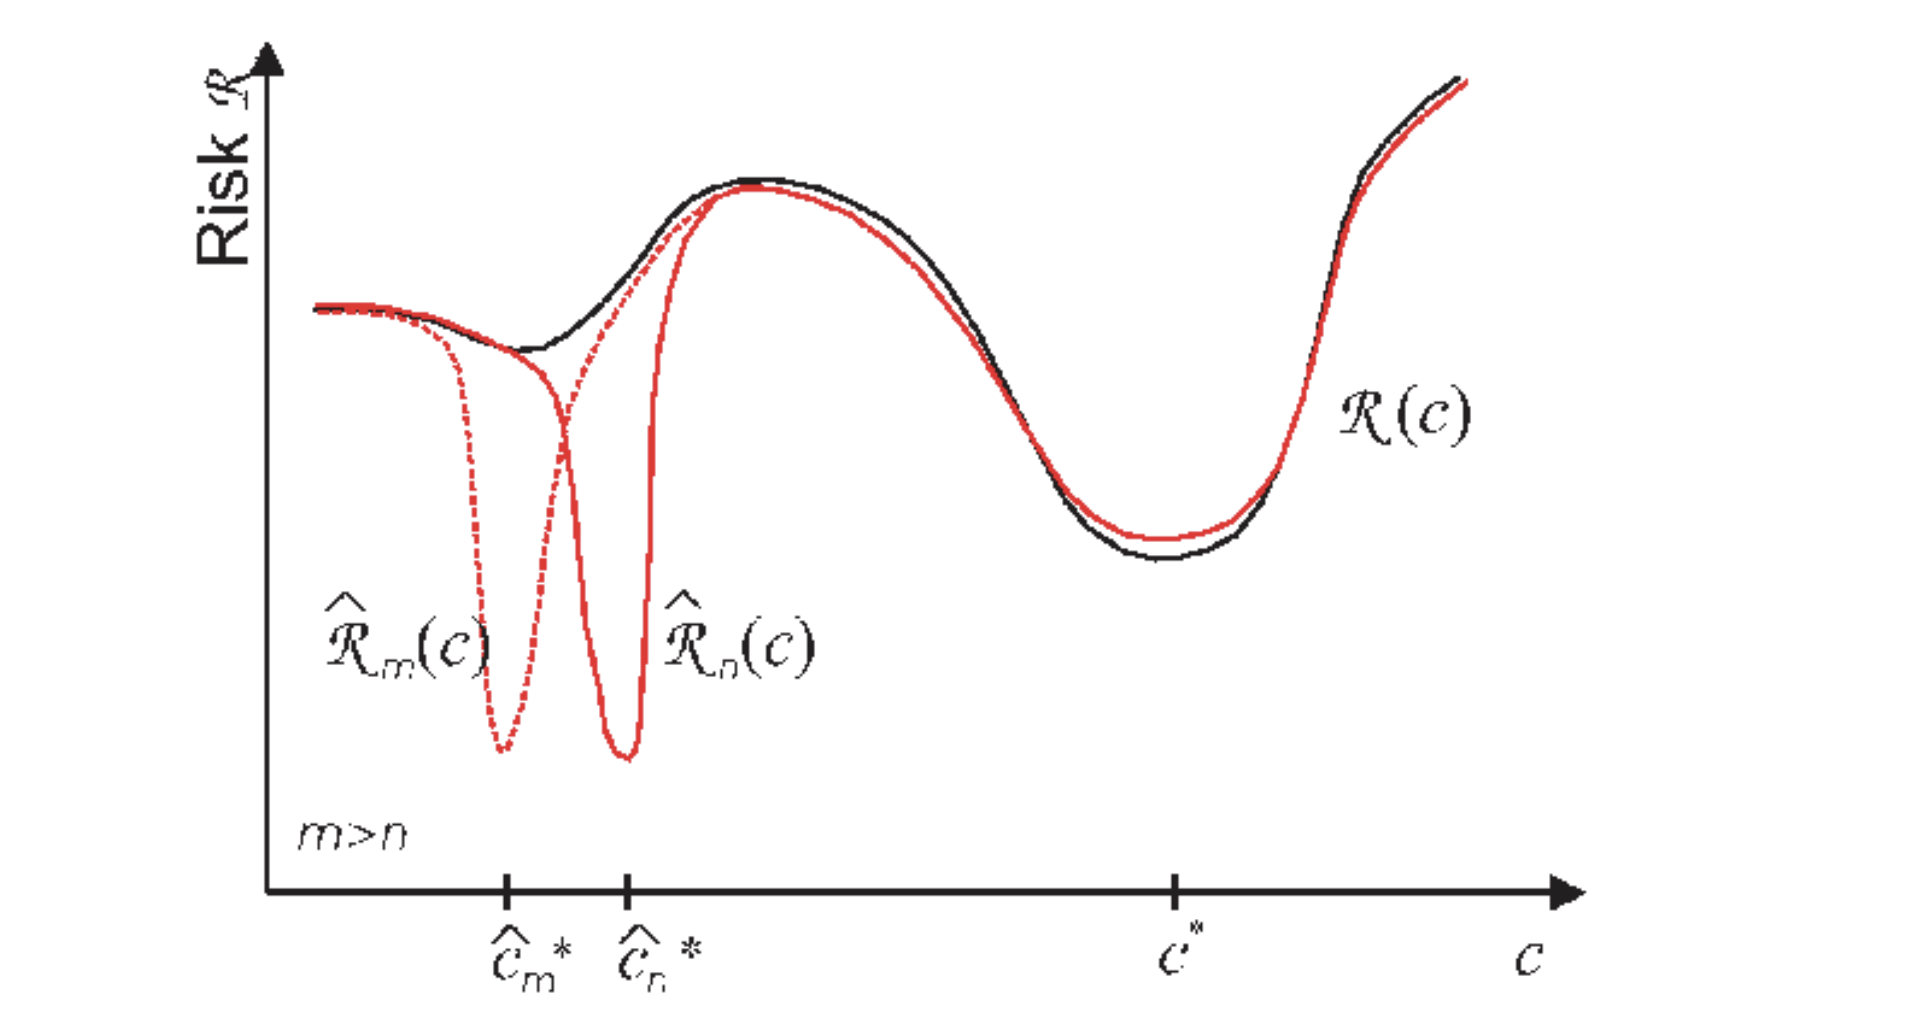
\includegraphics[width=0.6\textwidth]{img/erm.png}
\caption{In the worst case scenario pointwise convergence is not enough for the ERM algorithm to work. In Figure, $\mathcal{\hat{R}}_{n}(c)$ is  converging point-wise to $\mathcal{R}(c)$; however, since the convergence is not uniform, we have some $c$'s that do not converge for the current value of $n$ and cause the deviation in Figure. In this case, the ERM algorithm will pick the $\hat{c}$ that deviates the most $\mathcal{R}(c)$  thus, getting further and further away from the best classifier $c^*$.}
\end{figure}

But why do we need \textbf{uniform convergence}?\\ 
Overfitting the data implies that $\mathcal{\hat{R}}_{n}(c)$ and $\mathcal{R}(c)$ are very different, even if $\mathcal{\hat{R}}_{n}(c)$ is an unbiased
estimator of $\mathcal{R}(c)$!
Why will this happen? $\mathcal{\hat{R}}_{n}(c)$ is just the sample-average version of $\mathcal{R}(c)$, right? Is this contradicting the law
of large number that $\mathcal{\hat{R}}_{n}(c)$ converges to $\mathcal{R}(c)$?\\
It is true that $\mathcal{\hat{R}}_{n}(c)$ is an unbiased estimator of $\mathcal{R}(c)$ and yes indeed the law of large number is applicable
in this case. But a key requirement for using the law of large number is that we assume $c$ is fixed. Namely,
if the classifier $c$ is fixed, then the law of large number guarantees that the empirical risk $\mathcal{\hat{R}}_{n}(c)$ converges
to the true risk function $\mathcal{R}(c)$.
However, when we are finding the best classifier, we are consider many many many possible classifiers $c$.
Although for a given classifier $c$ the law of large number works, it may not work when we consider many
classifiers. The empirical risk minimization works if:
$$\sup_{c \in \mathcal{C}}{|\mathcal{R}(c) - \mathcal{\hat{R}}_{n}(c)|}  \overset{p}{\to} 0$$

Namely, the convergence is uniform for all classifiers in the collection that we are considering.


\end{document}